\begin{frame}
\frametitle{Scena: Demo}

\begin{columns}

\column{.5\textwidth}

\begin{figure}[ht]
    \centering
    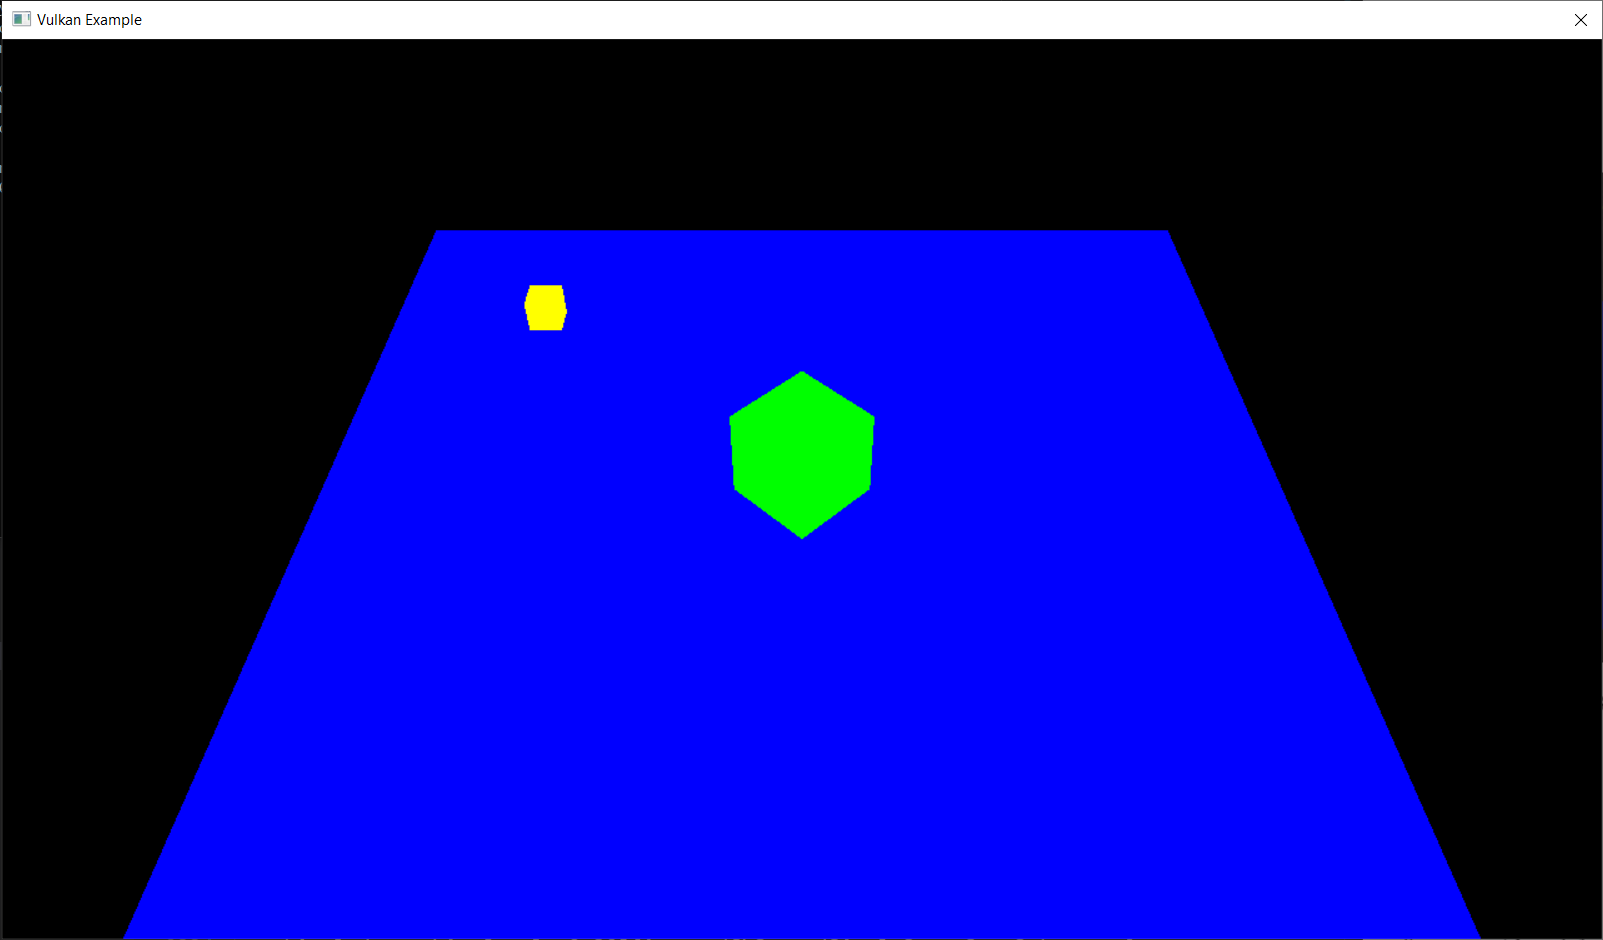
\includegraphics[scale=0.14]{images/SlidesScene/SimpleScene.png}
\end{figure}

\column{.5\textwidth}

\begin{figure}[ht]
    \centering
    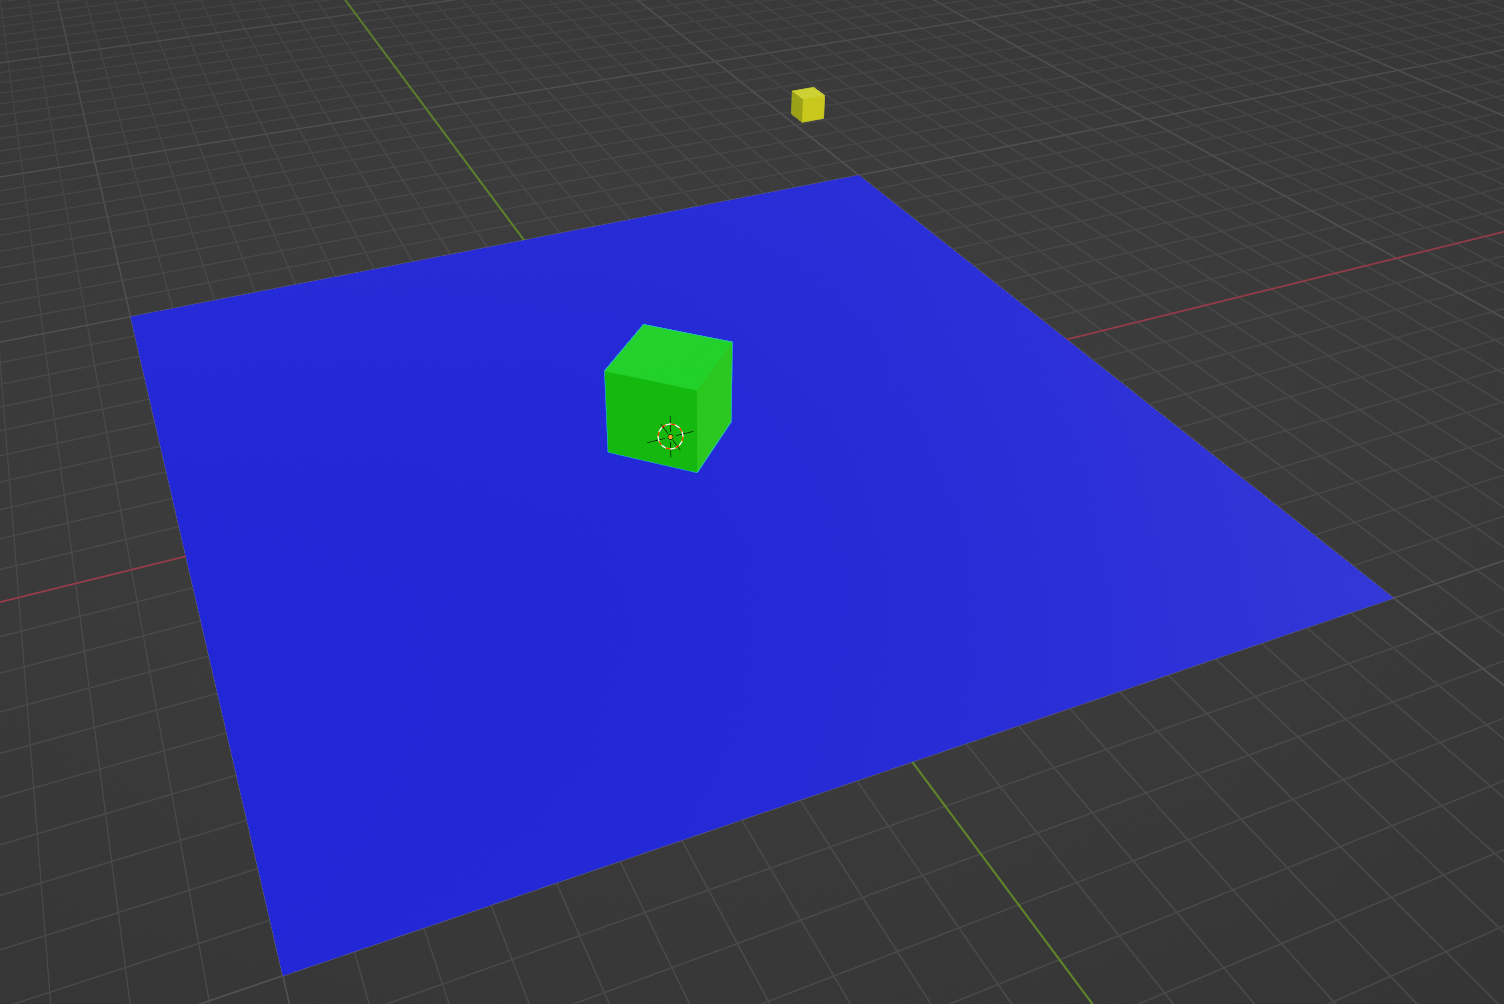
\includegraphics[scale=0.14]{images/SlidesScene/SimpleSceneSeenSetup.png}
\end{figure}

\end{columns}

\end{frame}

\begin{frame}
\frametitle{Scena}
\begin{itemize}
\item Organizziamo gli oggetti da renderizzare in una scena
\item Ogni oggetto ha una posizione, rotazione e scala (model matrix)
\item Uno o più oggetti condividono un vertex buffer e un pipeline state object
\item Più oggetti diversi possono usare gli stessi vertici e la stessa configurazione della pipeline
\item Ogni oggetto ha un proprio uniform buffer
\item Per renderizzare gli oggetti di una scena
\begin{itemize}
\item Usiamo il pipeline state object dell'oggetto
\item Usiamo il vertex buffer dell'oggetto
\item Usiamo lo uniform buffer dell'oggetto
\item Attiviamo la pipeline
\end{itemize}
\item Abbiamo una camera/occhio attraverso la quale guardiamo la scena (view e projection matrix)
\end{itemize}
\end{frame}
